\documentclass[10pt]{beamer}
\usetheme{metropolis}
\usepackage{booktabs}
\usepackage{tabularx}
\usepackage{calc}
\usepackage{tikz}
\usepackage[sfdefault]{FiraSans}
\usepackage[scaled]{FiraMono}
\usetikzlibrary{shapes.geometric, arrows, positioning, decorations.pathreplacing}

% Setup for faculty images
\newlength{\imageheight}
\setlength{\imageheight}{3.5cm}

% Define CSUF brand colors
\definecolor{titanblue}{HTML}{00244E}
\definecolor{mediumblue}{HTML}{0F3F8C}
\definecolor{skyblue}{HTML}{EBFBFF}
\definecolor{titanorange}{HTML}{FF7900}
\definecolor{titangray}{HTML}{F5F5F5}
\definecolor{titantext}{HTML}{222222}

% Customize metropolis theme colors
\setbeamercolor{normal text}{fg=titantext, bg=white}
\setbeamercolor{alerted text}{fg=titanorange}
\setbeamercolor{example text}{fg=mediumblue}

% Title page colors
\setbeamercolor{title}{fg=titanblue, bg=white}
\setbeamercolor{subtitle}{fg=mediumblue, bg=white}
\setbeamercolor{institute}{fg=titanorange, bg=white}
\setbeamercolor{date}{fg=titanblue, bg=white}

% Frame title colors
\setbeamercolor{frametitle}{fg=white, bg=titanblue}
\setbeamercolor{framesubtitle}{fg=mediumblue, bg=white}

% Block environment colors
\setbeamercolor{block title}{fg=white, bg=titanblue}
\setbeamercolor{block body}{fg=titantext, bg=skyblue!10}

% Item colors
\setbeamercolor{itemize item}{fg=titanorange}
\setbeamercolor{itemize subitem}{fg=mediumblue}
\setbeamercolor{itemize subsubitem}{fg=titanblue}

% Footer and header colors
\setbeamercolor{footer}{fg=titantext}
\setbeamercolor{header}{fg=titanblue}

% Customize fonts
\setbeamerfont{title}{size=\Large, series=\bfseries}
\setbeamerfont{frametitle}{size=\large, series=\bfseries}

% Simple title page template
\defbeamertemplate*{title page}{customized}[1][]
{
\vspace{1cm}
 {\usebeamerfont{title}\usebeamercolor[fg]{title}\inserttitle\par}
\vspace{0.5cm}
 {\usebeamerfont{subtitle}\usebeamercolor[fg]{subtitle}\insertsubtitle\par}
\vspace{0.5cm}
 {\usebeamerfont{date}\usebeamercolor[fg]{date}\insertdate\par}
\vfill
 {\insertinstitute\par}
}

% Add progress bar
\makeatletter
\setbeamertemplate{headline}{%
\begin{beamercolorbox}[wd=\paperwidth,ht=0.4cm,dp=0cm]{titanblue}%
\begin{tikzpicture}
\fill[titanorange] (0,0) rectangle (\the\paperwidth*\insertframenumber/\inserttotalframenumber,0.4cm);
\end{tikzpicture}%
\end{beamercolorbox}%
}
\makeatother

\begin{document}

\title{Understanding Politics and Public Policy}
\subtitle{Foundations and Core Concepts\\POSC 315: Introduction to Public Policy\\Lecture 8-1\\Decision Making (Part 1 of 3)}
\author{Dr. David P. Adams}
\date{Summer 2025}
\institute{California State University, Fullerton}

\maketitle

\begin{frame}{Today's Focus}
\begin{center}
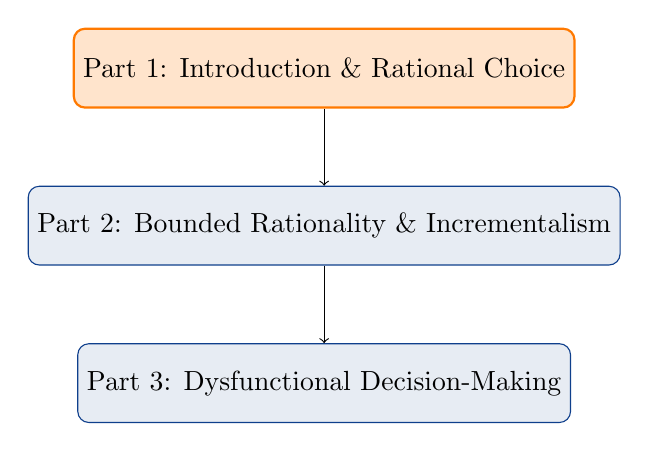
\begin{tikzpicture}[node distance=2cm]
% Define styles
\tikzstyle{current} = [rectangle, rounded corners, minimum width=3cm, minimum height=1cm, text centered, draw=titanorange, fill=titanorange!20, thick]
\tikzstyle{future} = [rectangle, rounded corners, minimum width=3cm, minimum height=1cm, text centered, draw=mediumblue, fill=mediumblue!10]

% Nodes
\node (part1) [current] {Part 1: Introduction \& Rational Choice};
\node (part2) [future, below of=part1] {Part 2: Bounded Rationality \& Incrementalism};
\node (part3) [future, below of=part2] {Part 3: Dysfunctional Decision-Making};

% Arrows
\draw[->] (part1) -- (part2);
\draw[->] (part2) -- (part3);
\end{tikzpicture}
\end{center}
\end{frame}

\begin{frame}{The Decision-Making Process}
\begin{center}
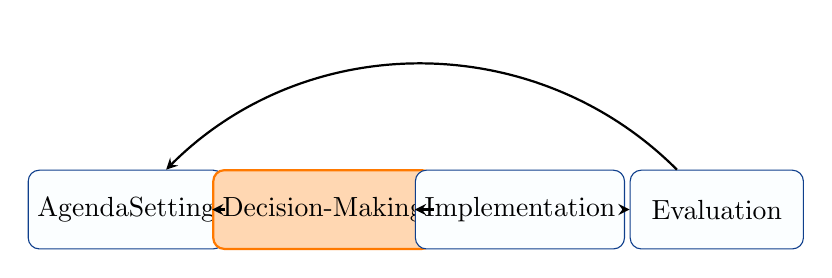
\begin{tikzpicture}[node distance=2.5cm]
% Define styles
\tikzstyle{stage} = [rectangle, rounded corners, minimum width=2.2cm, minimum height=1cm, text centered, draw=mediumblue, fill=skyblue!20]
\tikzstyle{highlight} = [rectangle, rounded corners, minimum width=2.2cm, minimum height=1cm, text centered, draw=titanorange, fill=titanorange!30, thick]
\tikzstyle{arrow} = [thick,->,>=stealth]

% Nodes
\node (agenda) [stage] {Agenda\\Setting};
\node (decision) [highlight, right of=agenda] {Decision-\\Making};
\node (implement) [stage, right of=decision] {Implementation};
\node (evaluate) [stage, right of=implement] {Evaluation};

% Arrows
\draw[arrow] (agenda) -- (decision);
\draw[arrow] (decision) -- (implement);
\draw[arrow] (implement) -- (evaluate);
\draw[arrow] (evaluate) to [bend right=45] (agenda);
\end{tikzpicture}
\end{center}

\vspace{1cm}
\begin{itemize}
\item Policy design in the \textcolor{titanorange}{\textbf{Alternative Selection}} stage requires decisions about what ``tools'' to adopt
\item Decision-making also permeates ongoing policy design, budgeting, implementation, and evaluation
\end{itemize}
\end{frame}

\begin{frame}{Understanding Decision Points}
\begin{columns}
\begin{column}{0.5\textwidth}
\textbf{Key Considerations}
\begin{itemize}
\item Decisions occur throughout the policy process
\item Multiple decision points at each stage
\item Different actors involved at different points
\end{itemize}
\end{column}
\begin{column}{0.5\textwidth}
\begin{block}{Complexity Spectrum}
\textbf{Complex:} What is the best way to reduce traffic fatalities?

\vspace{0.3cm}
\textbf{Simple:} Should we build a new bridge?
\end{block}

\vspace{0.3cm}
\small{Our constitutional system intentionally slows policy-oriented decision-making.}
\end{column}
\end{columns}
\end{frame}

\begin{frame}{Decision-Making Theories}
Three primary theoretical frameworks to understand how decisions are made in policy contexts:

\vspace{1cm}
\begin{center}

\begin{tikzpicture}[node distance=3cm]
\tikzstyle{theory} = [rectangle, rounded corners, minimum width=2.8cm, minimum height=1.5cm, text centered, draw=mediumblue]

\node (rational) [theory, fill=mediumblue!10] {\textbf{Rational Choice}\\{\footnotesize Optimizing decisions based on complete information}};
\node (bounded) [theory, fill=mediumblue!20, right of=rational] {\textbf{Bounded Rationality}\\{\footnotesize Satisficing with limited information \& capacity}};
\node (incremental) [theory, fill=mediumblue!10, right of=bounded] {\textbf{Incrementalism}\\{\footnotesize Making small changes from the status quo}};

\end{tikzpicture}
\end{center}
\end{frame}

\begin{frame}{Rational Choice Theory}
\begin{block}{Foundation}
The Rational-Comprehensive Model is the starting point for many decision-making theories.
\end{block}

\vspace{0.5cm}
\begin{columns}
\begin{column}{0.5\textwidth}
\textbf{Key Assumptions}
\begin{itemize}
\item All important factors are considered
\item Analysis of goals separate from tools
\item Goals are isolated before tools are considered
\end{itemize}
\end{column}
\begin{column}{0.5\textwidth}
\textbf{Definition of ``Good'' Policy}

A \emph{good} policy is the \emph{technically} best policy that maximizes benefits and minimizes costs.
\end{column}
\end{columns}
\end{frame}

\begin{frame}{The ``Economic Man''}
Rational Choice depends on the existence of a perfectly rational actor:

\vspace{0.5cm}
\begin{center}
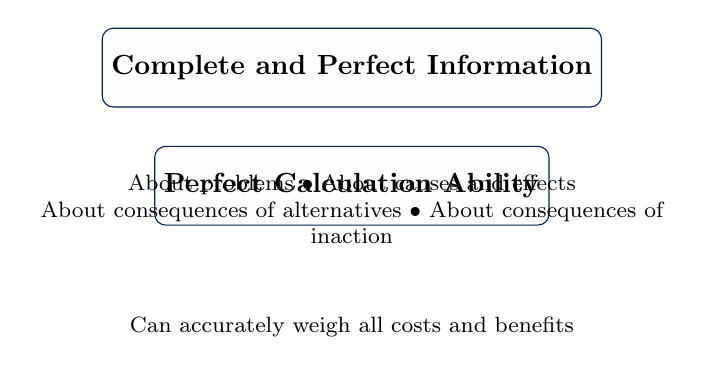
\begin{tikzpicture}[node distance=1.5cm]
\tikzstyle{req} = [rectangle, rounded corners, minimum width=5cm, minimum height=1cm, text centered, draw=titanblue, fill=skyblue!15]

\node (info) [req] {\textbf{Complete and Perfect Information}};
\node (calc) [req, below of=info] {\textbf{Perfect Calculation Ability}};

% Detail boxes
\node (infodetail) [below of=info, yshift=-0.3cm] {
\begin{minipage}{8cm}
\centering
\footnotesize
About problems $\bullet$ About causes and effects\\
About consequences of alternatives $\bullet$ About consequences of inaction
\end{minipage}
};

\node (calcdetail) [below of=calc, yshift=-0.3cm] {
\begin{minipage}{8cm}
\centering
\footnotesize
Can accurately weigh all costs and benefits
\end{minipage}
};

\end{tikzpicture}
\end{center}
\end{frame}

\begin{frame}{Optimization in Rational Choice}
\begin{block}{Core Principle}
\begin{itemize}
\item The rational actor chooses the option that \textcolor{titanorange}{\textbf{maximizes benefits}} and \textcolor{titanorange}{\textbf{minimizes costs}}
\item All alternatives are considered comprehensively
\item Decisions achieve maximum social gain
\end{itemize}
\end{block}

\vspace{0.5cm}
\textbf{Limitations of Rational Choice}
\begin{itemize}
\item Information is never complete or perfect
\item Costs and benefits are difficult to predict accurately
\item Decision-makers face resource constraints
\item Bureaucracy helps make the model more realistic
\end{itemize}
\end{frame}

\begin{frame}{Six Steps to Rational Choice}
\begin{center}
\begin{tikzpicture}[node distance=0.8cm]
\tikzstyle{step} = [rectangle, rounded corners, minimum width=8cm, minimum height=0.8cm, text centered, draw=mediumblue, fill=skyblue!10]

\node (step1) [step] {1. \textcolor{titanorange}{\textbf{Define the problem}} - What exactly are we trying to solve?};
\node (step2) [step, below of=step1] {2. \textcolor{titanorange}{\textbf{Identify decision criteria}} - What factors matter in making this decision?};
\node (step3) [step, below of=step2] {3. \textcolor{titanorange}{\textbf{Weight the criteria}} - How important is each factor?};
\node (step4) [step, below of=step3] {4. \textcolor{titanorange}{\textbf{Generate alternatives}} - What are all possible solutions?};
\node (step5) [step, below of=step4] {5. \textcolor{titanorange}{\textbf{Rate alternatives}} - How does each solution perform on each criterion?};
\node (step6) [step, below of=step5] {6. \textcolor{titanorange}{\textbf{Compute optimal decision}} - Which solution maximizes benefits?};

\end{tikzpicture}
\end{center}
\end{frame}

\begin{frame}{Rational Choice: Example}
\begin{block}{Case: Highway Safety Policy}
\end{block}

\begin{columns}
\begin{column}{0.5\textwidth}
\textbf{Problem Definition}

Reduce traffic fatalities on interstate highways by 50\% within 5 years

\vspace{0.5cm}
\textbf{Criteria \& Weights}
\begin{itemize}
\item Effectiveness (40\%)
\item Implementation cost (30\%)
\item Time to implement (20\%)
\item Public acceptance (10\%)
\end{itemize}
\end{column}
\begin{column}{0.5\textwidth}
\textbf{Alternatives Analyzed}
\begin{enumerate}
\item Lower speed limits
\item Increase enforcement
\item \textcolor{titanorange}{\textbf{Mandate vehicle safety features}}
\item Improve road design
\item Enhance driver education
\end{enumerate}

\vspace{0.5cm}
\textbf{Decision}

After comprehensive analysis, the highest-scoring option is selected as it provides optimal benefit-cost ratio.
\end{column}
\end{columns}
\end{frame}

\begin{frame}{Rational Choice: Visualization}
\begin{center}
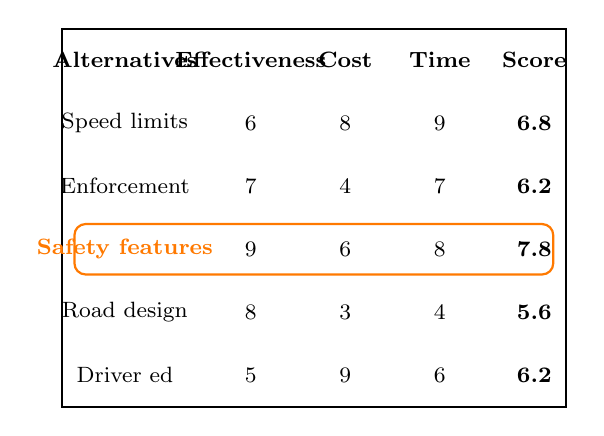
\begin{tikzpicture}[scale=0.8]
% Create a decision matrix visualization
\draw[thick] (0,0) rectangle (8,6);

% Headers
\node at (1,5.5) {\footnotesize \textbf{Alternatives}};
\node at (3,5.5) {\footnotesize \textbf{Effectiveness}};
\node at (4.5,5.5) {\footnotesize \textbf{Cost}};
\node at (6,5.5) {\footnotesize \textbf{Time}};
\node at (7.5,5.5) {\footnotesize \textbf{Score}};

% Data rows
\node[align=left] at (1,4.5) {\footnotesize Speed limits};
\node[align=left] at (1,3.5) {\footnotesize Enforcement};
\node[align=left] at (1,2.5) {\footnotesize \textcolor{titanorange}{\textbf{Safety features}}};
\node[align=left] at (1,1.5) {\footnotesize Road design};
\node[align=left] at (1,0.5) {\footnotesize Driver ed};

% Scores (simplified)
\foreach \y/\eff/\cost/\time/\total in {4.5/6/8/9/6.8, 3.5/7/4/7/6.2, 2.5/9/6/8/7.8, 1.5/8/3/4/5.6, 0.5/5/9/6/6.2} {
    \node at (3,\y) {\footnotesize \eff};
    \node at (4.5,\y) {\footnotesize \cost};
    \node at (6,\y) {\footnotesize \time};
    \node at (7.5,\y) {\footnotesize \textbf{\total}};
}

% Highlight winner
\draw[titanorange, thick, rounded corners] (0.2,2.1) rectangle (7.8,2.9);

\end{tikzpicture}
\end{center}
\end{frame}

\begin{frame}{Key Takeaways: Rational Choice}
\begin{center}
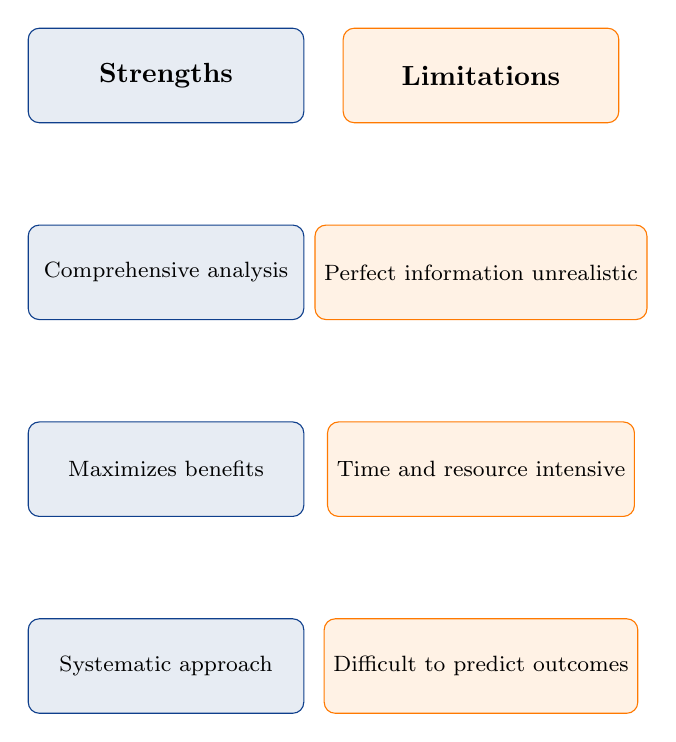
\begin{tikzpicture}[node distance=2cm]
\tikzstyle{pro} = [rectangle, rounded corners, minimum width=3.5cm, minimum height=1.2cm, text centered, draw=mediumblue, fill=mediumblue!10]
\tikzstyle{con} = [rectangle, rounded corners, minimum width=3.5cm, minimum height=1.2cm, text centered, draw=titanorange, fill=titanorange!10]

\node (prohead) [pro] {\textbf{Strengths}};
\node (conhead) [con, right of=prohead, xshift=2cm] {\textbf{Limitations}};

\node (pro1) [pro, below of=prohead, yshift=-0.5cm] {\footnotesize Comprehensive analysis};
\node (pro2) [pro, below of=pro1, yshift=-0.5cm] {\footnotesize Maximizes benefits};
\node (pro3) [pro, below of=pro2, yshift=-0.5cm] {\footnotesize Systematic approach};

\node (con1) [con, below of=conhead, yshift=-0.5cm] {\footnotesize Perfect information unrealistic};
\node (con2) [con, below of=con1, yshift=-0.5cm] {\footnotesize Time and resource intensive};
\node (con3) [con, below of=con2, yshift=-0.5cm] {\footnotesize Difficult to predict outcomes};

\end{tikzpicture}
\end{center}
\end{frame}

\begin{frame}{Looking Ahead}
\begin{center}
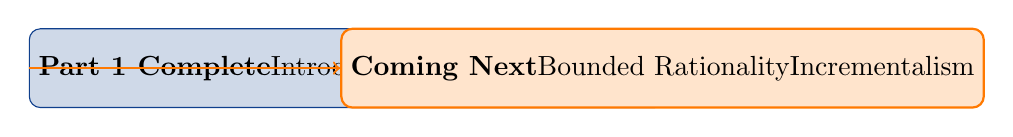
\begin{tikzpicture}[node distance=2cm]
\tikzstyle{completed} = [rectangle, rounded corners, minimum width=4cm, minimum height=1cm, text centered, draw=mediumblue, fill=mediumblue!20]
\tikzstyle{next} = [rectangle, rounded corners, minimum width=4cm, minimum height=1cm, text centered, draw=titanorange, fill=titanorange!20, thick]

\node (current) [completed] {\textbf{Part 1 Complete}\\Introduction \& Rational Choice};
\node (part2) [next, right of=current, xshift=2cm] {\textbf{Coming Next}\\Bounded Rationality\\Incrementalism};

\draw[->, thick, titanorange] (current) -- (part2);

\end{tikzpicture}
\end{center}

\vspace{1cm}
\textbf{Next time we'll explore:}
\begin{itemize}
\item Herbert Simon's ``Administrative Man''
\item The concept of ``satisficing''
\item Charles Lindblom's ``Muddling Through''
\item When incremental change makes sense
\end{itemize}
\end{frame}

\end{document}